\documentclass[margin = 2cm]{article}

\usepackage{polski}
\usepackage{graphicx}
\usepackage{listings} %listingi kodu
\usepackage{array}
\usepackage{float}
\usepackage{amsmath}
\usepackage{multicol} %kolumny
\usepackage[margin=0.8in]{geometry}
\usepackage{gensymb} %stopnie (symbol)

\graphicspath{ {./images/} } %obrazy

\begin{document} %tytuł
\title{\textbf{Sprawozdanie z zajęć numer 1,2,3 \\Systemy i sieci przemysłowe}} % \\ robi nową linię
\author{Maciej Misiewicz\\215305 \and Oskar Zieliński\\215373 \and Dariusz Witek vel Witkowski\\215364 \and Szymon Panek\\215319}

\maketitle


\newpage
\tableofcontents
\newpage

\section{Laboratorium 1}
\section{Laboratorium 2}
	\subsection{Cel ćwiczenia}
	Celem ćwiczenia było zapoznanie się z komunikacją za pomocą protokołu CAN na przykładzie połączenia z częścią składową robota hipermobilnego Wheeeler. Ćwiczenie obejmowało wysyłanie rozkazów oraz odbieranie informacji od lokalnego sterownika za pomocą ramek danych.
	\subsection{Realizacja ćwiczenia}
	\subsubsection{Konfiguracja połączenia z robotem}
	Konfiguracja połączenia z robotem ograniczała się do określenia dwóch parametrów - prędkości transmisji jako 1Mbit/s oraz formatu identyfikatora jako format extended.
	\begin{figure}[H]
		\centering
		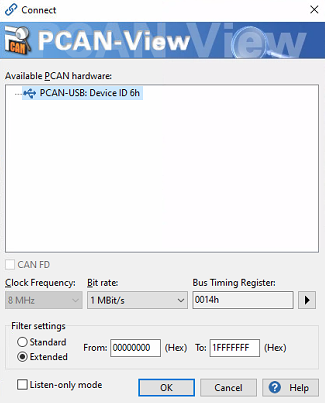
\includegraphics[width=0.5\textwidth]{0}
		\caption{Okno nawiązywania połączenia}
	\end{figure}
	Po udanym połączeniu zostały odebrane trzy ramki danych.
	\begin{figure}[H]
		\centering
		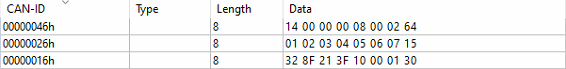
\includegraphics[width=0.9\textwidth]{0_1}
		\caption{Odebrane ramki danych}
	\end{figure}
	\begin{figure}[H]
		\centering
		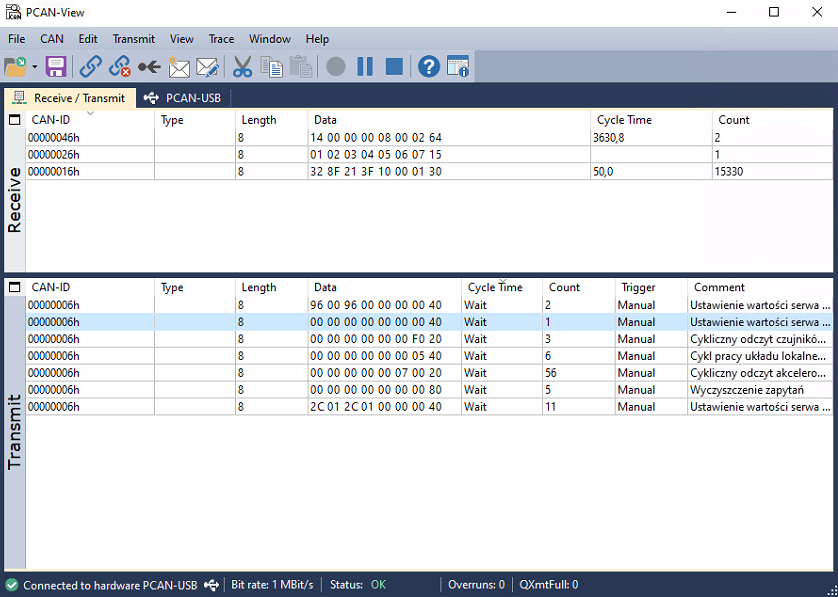
\includegraphics[width=0.9\textwidth]{interfejs}
		\caption{Widok interfejsu w programie PCANView.}
	\end{figure}
	\begin{figure}[H]
		\centering
		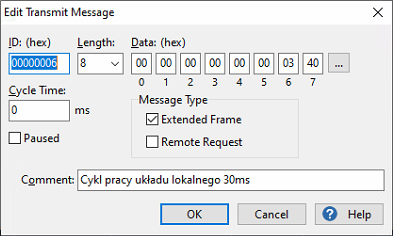
\includegraphics[width=0.6\textwidth]{edytorinstrukcji}
		\caption{Kreator rozkazów}
	\end{figure}
	\subsubsection{Ustawienie cyklu pracy układu lokalnego 30ms}
	\label{a}
	Ustawienie cyklu pracy układu lokalnego odbywa się za pomocą 6 bajtu, podana w nim wartość w zakresie 2-20 (dec) zwiększających cykl co 10ms. Bajt 7 odpowiada za ustawienie zadanych wartości w instrukcji.  Ramka realizujaca zadanie wygląda następująco:
	
	00000006h	00 00 00 00 00 00 03 40
	
	\begin{figure}[H]
		\centering
		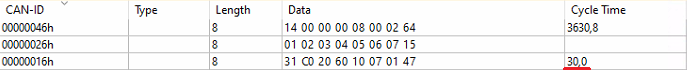
\includegraphics[width=0.9\textwidth]{30ms}
	\end{figure}
	
	\subsubsection{Ustawienie cyklicznego odczytu danych z akcelerometru}
	Ustawienie odczytu danych z akcelerometru odbywa się za pomocą 4 bajtu. Ustawiona wartość 07 jest składową odczytu osi X, Y i Z. Bajt 7 odpowiada za cykliczne odczytywanie pomiarów. Ramka realizujaca zadanie wygląda następująco:
	
	00000006h	00 00 00 00 00 07 00 20
	\subsubsection{Ustawienie cyklicznego odczytu danych z czujników odległości}
	Ustawienie odczytu danych z czujników odległości odbywa się za pomocą 6 bajtu. Ustawiona wartość F0 jest składową adresów 4 czujników odległości. Bajt 7 odpowiada za cykliczne odczytywanie pomiarów. 
	
	00000006h	00 00 00 00 00 00 F0 20
	\subsubsection{Zmiana położenie serwa 1 i serwa 2}
	Zakres roboczy obu serw mieści się między 0 a 300 (dec), naszym zadaniem było ustawienie 3 zadanych pozycji: minimalnej, środkowej oraz maksymalnej. Wysterowanie pojedynczego serwa odbywa się przy pomocy dwóch bajtów. Dla serwa 1 jest to bajt0 oraz bajt1, natomiast dla    serwa 2  bajt2 oraz bajt3.
	
	max
	
	00000006h	2C 01 2C 01 00 00 00 40
	\begin{figure}[H]
		\centering
		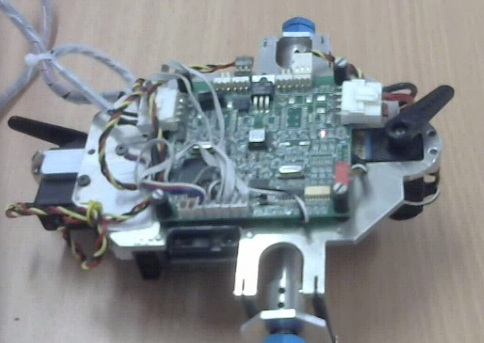
\includegraphics[width=0.9\textwidth]{max}
	\end{figure}
	middle
	
	00000006h	96 00 96 00 00 00 00 40
	\begin{figure}[H]
		\centering
		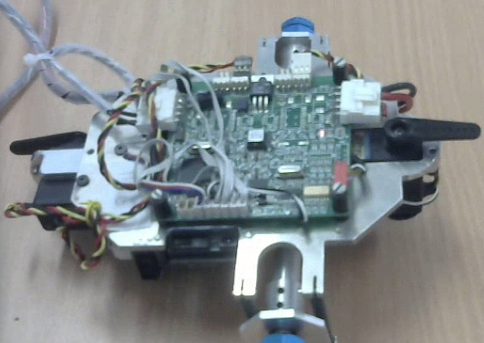
\includegraphics[width=0.9\textwidth]{middle}
	\end{figure}
	min
	
	00000006h	00 00 00 00 00 00 00 40
	\begin{figure}[H]
		\centering
		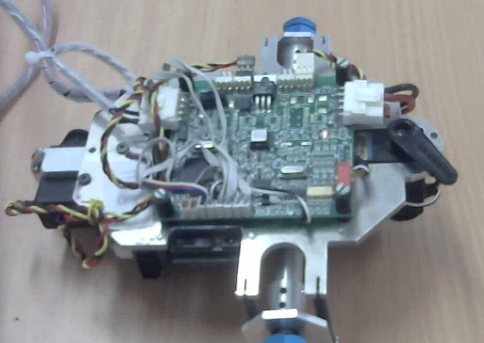
\includegraphics[width=0.9\textwidth]{min}
	\end{figure}
	\subsubsection{Zmiana cyklu pracy układu lokalnego na 50ms}
	Analogicznie do punktu \ref{a}, zmianie uległa jedynie zadana długość cyklu.
	
	00000006h	00 00 00 00 00 00 05 40
	\begin{figure}[H]
		\centering
		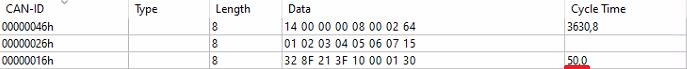
\includegraphics[width=0.9\textwidth]{50ms}
	\end{figure}
	\subsection{Wnioski i spostrzeżenia}
	Oprogramowanie PCANView jest łatwym, czytelnym i intuicyjnym narzędziem. Bezpośrednio pokazuje komunikację za pomocą ramek, dzieląc je na przychodzące i wysyłane. Jest dobrym programem do testowania oraz podglądu transmisji protokołem CAN. Zaletą jest także możliwość wyboru sposobu wysyłania rozkazów. Możemy wysłać ramkę pojedynczo manualnie lub wysyłać cyklicznie w zadanym interwale. Program sygnalizuje status połączenia w protokole. 
\section{Laboratorium 3}
	\subsection{Cel ćwiczenia}
Zapoznanie się z podstawowymi pojęciami w środowisku programowym LabVIEW oraz ze strukturą FPGA i Real-Time sterownika CompactRIO.
	\subsection{Realizacja ćwiczenia}
  		\subsubsection{Uzupełnienie brakującej części kodu, tak aby możliwe było sterowanie pozostałymi złączami}
Uzupełnienie brakującej części programu polegało na dodaniu suwaków zadających pozycję poszczególnych złączy manipulatora, których skala została odpowiednio dobrana do zakresu pracy złącz. Dane odbierane z dodanych elementów interfejsu zostają przesłane do bloku FPGA oraz udostępniane jako zmienne globalne środowiska RIO. W celu umożliwienia kontroli z poziomu panelu HMI, kod odpowiedzialny za uaktualnianie wartości położenia został objęty blockiem case-if.
	\begin{figure}[H]
		\centering
		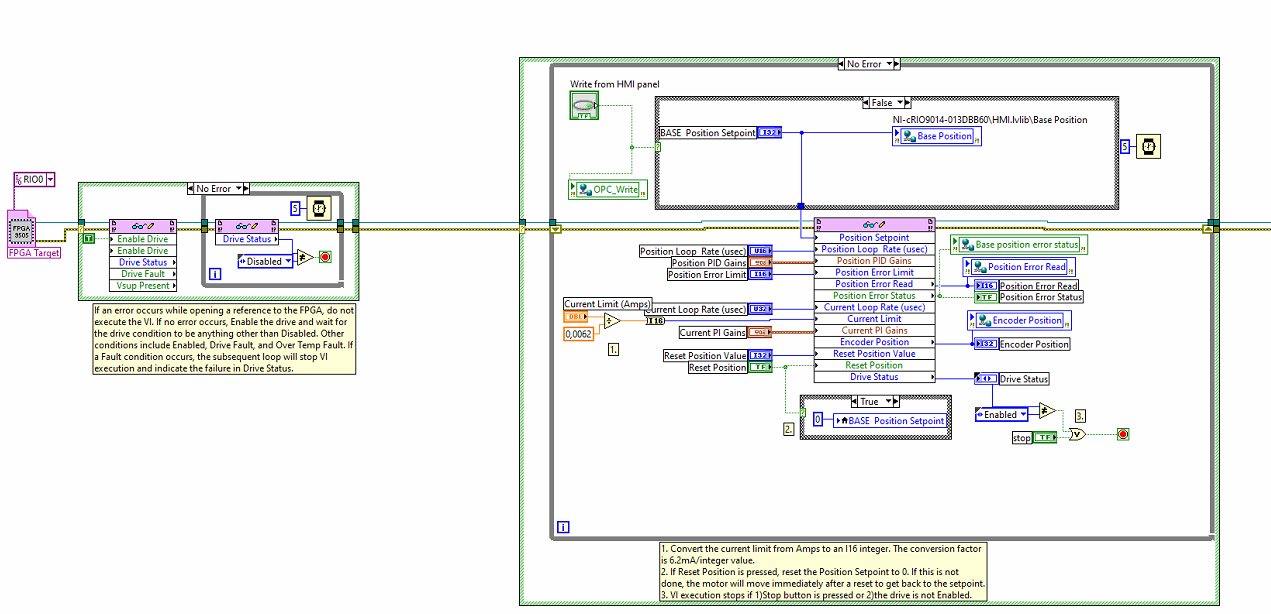
\includegraphics[width=0.9\textwidth]{3_1}
		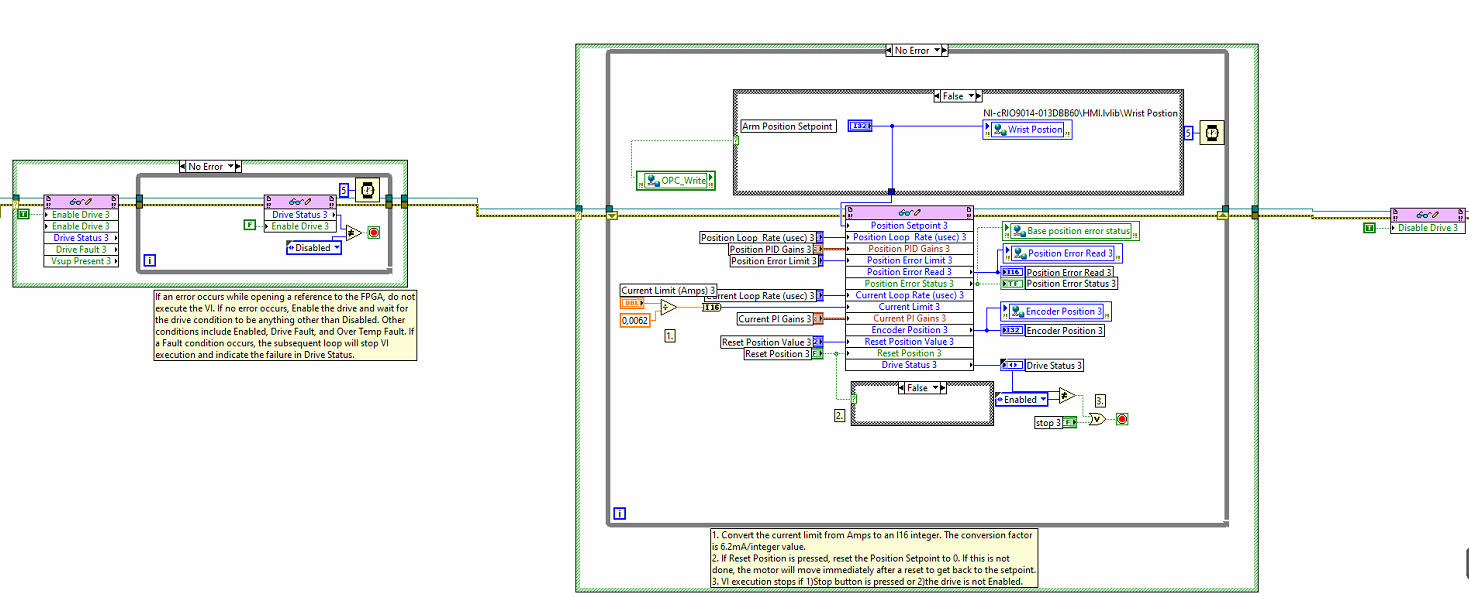
\includegraphics[width=0.9\textwidth]{3_2}
		\caption{Realizacja połączenia panelu kontrolnego użytkownika z blokiem FPGA}
	\end{figure}

	\begin{figure}[H]
		\centering
		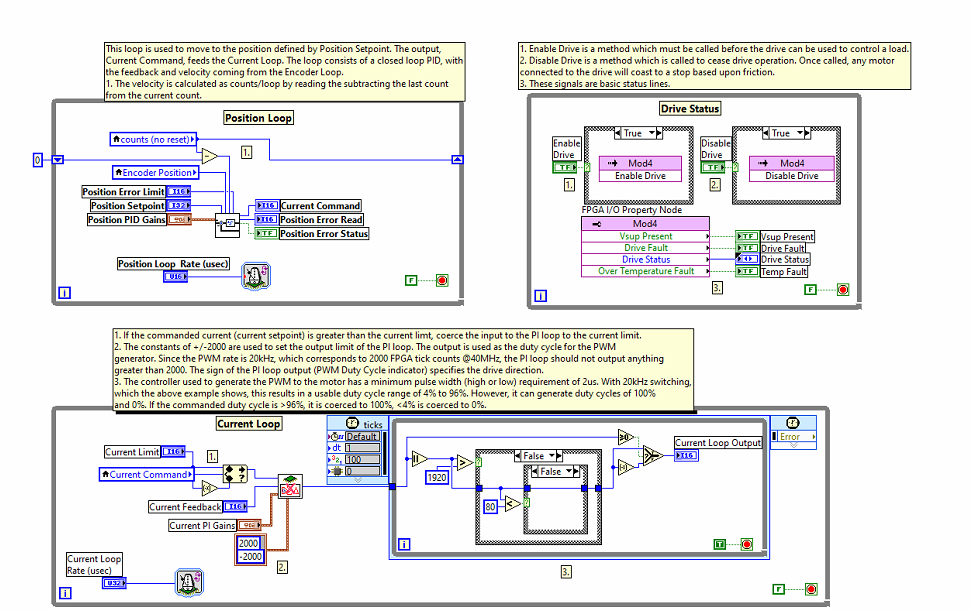
\includegraphics[width=0.9\textwidth]{3_3}

		\caption{Struktura bloku FPGA odpowiedzialnego za sterowanie złączami.}
	\end{figure}
	\begin{figure}[H]
		\centering
		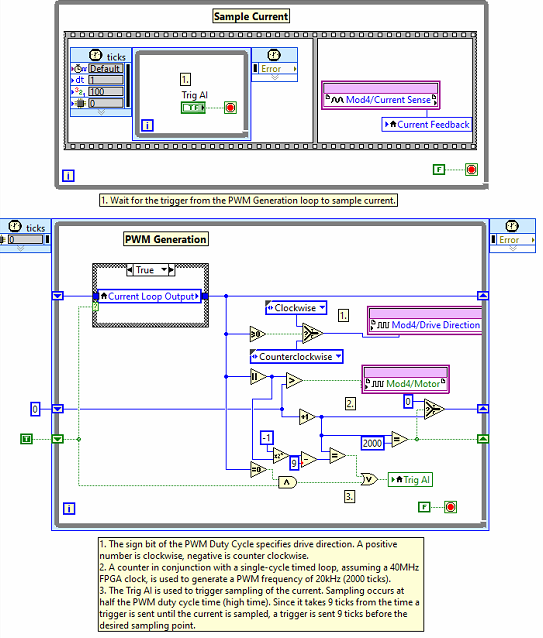
\includegraphics[width=0.5\textwidth]{3_4}
		\caption{Struktura bloku FPGA odpowiedzialnego za sterowanie złączami.}
	\end{figure}
	\begin{figure}[H]
		\centering
		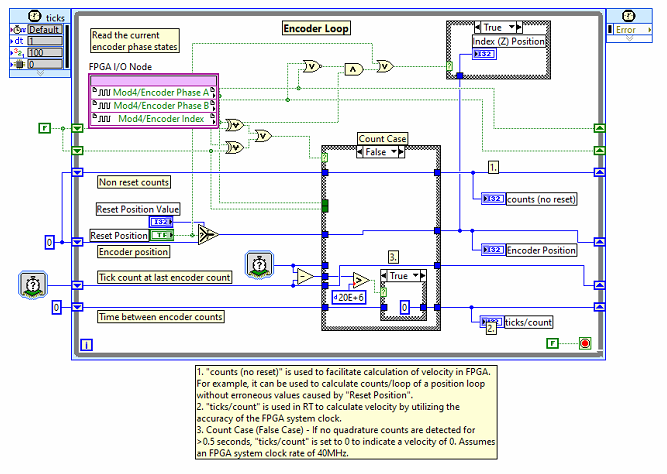
\includegraphics[width=0.7\textwidth]{3_5}
		\caption{Struktura bloku FPGA odpowiedzialnego za sterowanie złączami.}
	\end{figure}
		\subsubsection{Dobranie nastaw regulatorów PID dla ramienia oraz nadgarstka robota}
	\begin{figure}[H]
		\centering
		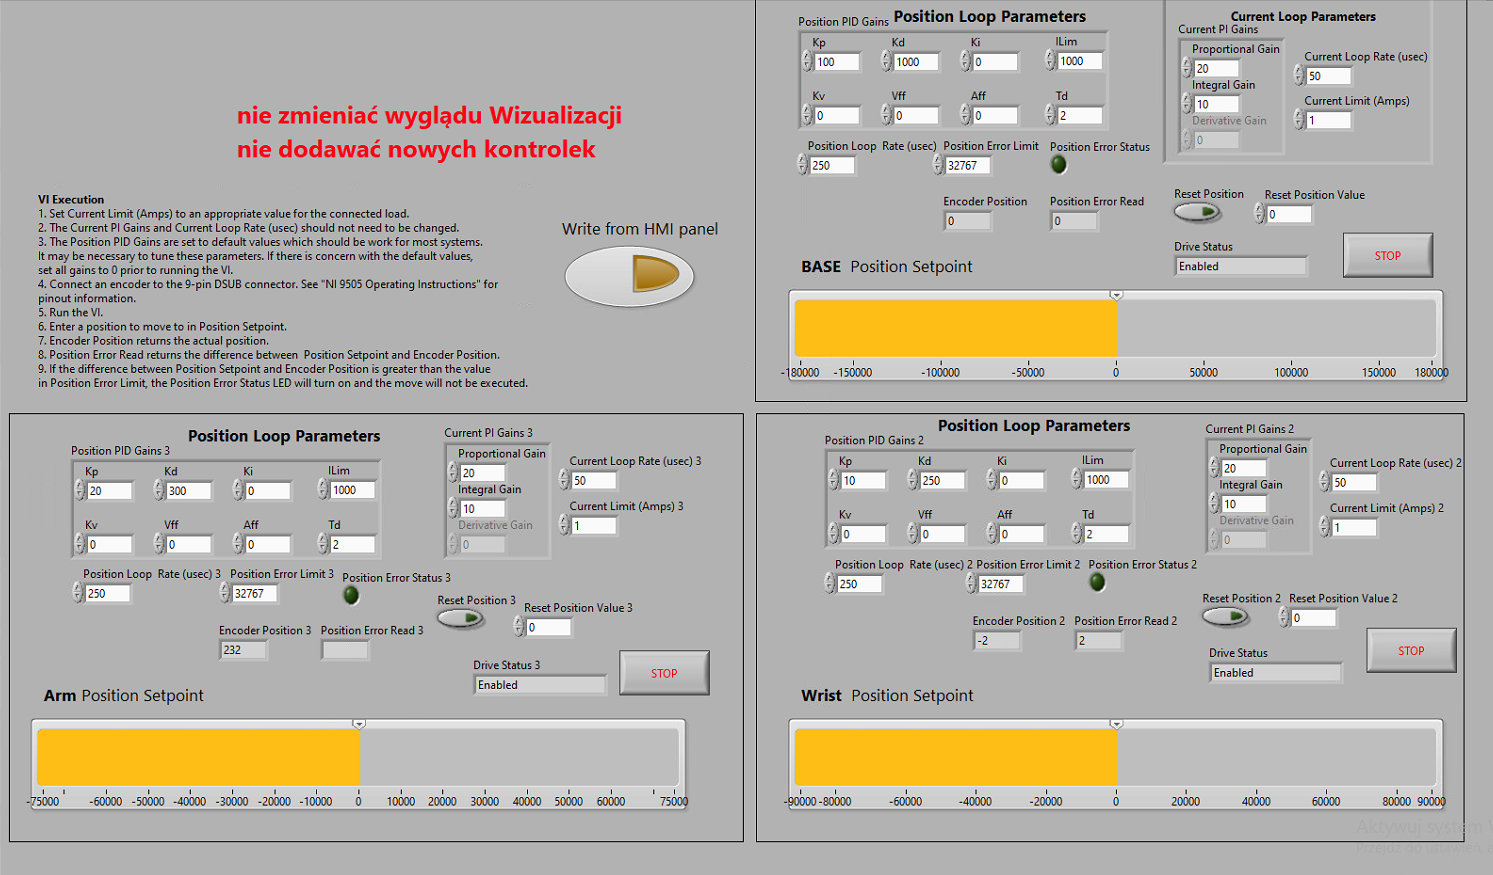
\includegraphics[width=0.9\textwidth]{3_panel}
		\caption{Widok panelu kontrolnego sterowników poszczególnych złącz wraz z dobranymi nastawami regulatorów}
	\end{figure}
Z poziomu panelu jesteśmy w stanie zadać pozycje poszczególnych złącz przy pomocy suwaków. Przy użyciu tego panelu jesteśmy w stanie zmieniać nastawy regulatorów PID poszczególnych złącz manipulatora. Za pomocą przełącznika możemy udzielić dostępu do sterowania z poziomu panelu HMI, jednocześnie odcinając możliwość zmiany parametrów z poziomu panel sterowania.
	\subsection{Wnioski i spostrzeżenia}
Nastawy regulatorów zostały dobrane w taki sposób, aby ruch poszczególnych złącz manipulatora do pozycji zadanych odbywał się w jak najkrótszym czasie jednocześnie nie wywołując oscylacji. 

Za szybka zmiana zadanego położenia powodowała gwałtowny skok błędu odczytu enkodera, który był sygnalizowany przez kontrolkę w panelu użytkownika. Błąd ten skutkował zatrzymaniem pracy złącza, czego efektem było niezrealizowanie zadanego położenia.

Podczas realizacji ćwiczenia zauważyliśmy, że zmienne pozycyjne nadgarstka i ramienia są ze sobą zamienione. Może to być spowodowane błędem definicji zmiennych globalnych lub niewłaściwym podłączeniem silników do sterownika.


\end{document}